% How the ear takes the rise: a linear attack and a Moog (exponential-approach) attack of the same nominal time T,
% once as the code writes them (amplitude) and once as the ear counts them (decibels).
% Curves are analytic: linear a = t/T ; Moog a = 1 - exp(-3 t/T), the 95 % point at t = T.
% Compile: pdflatex heard-rise-linear-vs-moog.tex ; SVG via PyMuPDF (dvisvgm --pdf is broken on this Mac).
\documentclass[border=6pt]{standalone}
\usepackage{tikz}
\usepackage{pgfplots}
\pgfplotsset{compat=1.16}
\definecolor{ink}{RGB}{51,51,51}
\definecolor{moog}{RGB}{180,67,47}
\definecolor{lin}{RGB}{90,90,90}
\begin{document}
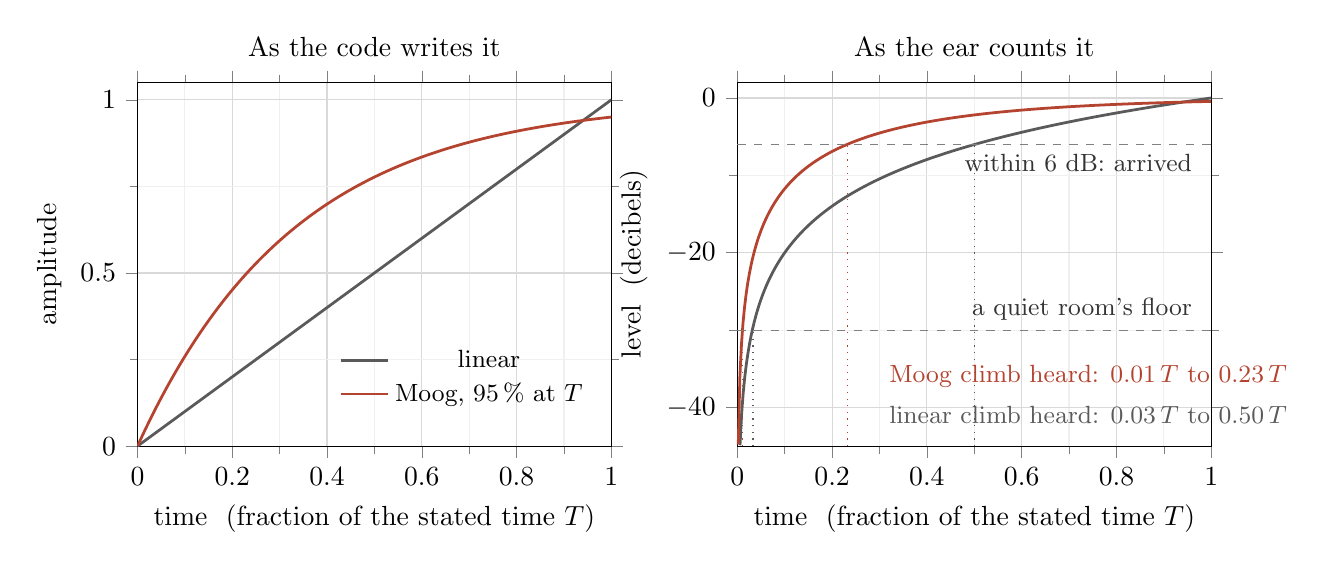
\begin{tikzpicture}
\begin{axis}[
  name=amp, width=7.6cm, height=6.2cm,
  xlabel={time \ (fraction of the stated time $T$)},
  ylabel={amplitude},
  title={As the code writes it},
  xmin=0, xmax=1, ymin=0, ymax=1.05,
  grid=both, major grid style={gray!30}, minor grid style={gray!12}, minor tick num=1,
  tick align=outside, domain=0:1, samples=200,
  every axis plot/.append style={line width=1pt},
  legend style={at={(0.97,0.08)}, anchor=south east, draw=none, fill=none, font=\small},
]
  \addplot[lin] {x};
  \addlegendentry{linear}
  \addplot[moog] {1-exp(-3*x)};
  \addlegendentry{Moog, 95\,\% at $T$}
\end{axis}
\begin{axis}[
  name=db, at={(amp.east)}, anchor=west, xshift=1.6cm, clip=false,
  width=7.6cm, height=6.2cm,
  xlabel={time \ (fraction of the stated time $T$)},
  ylabel={level \ (decibels)},
  title={As the ear counts it},
  xmin=0, xmax=1, ymin=-45, ymax=2,
  grid=both, major grid style={gray!30}, minor grid style={gray!12}, minor tick num=1,
  tick align=outside, domain=0.002:1, samples=300,
  every axis plot/.append style={line width=1pt},
]
  \addplot[lin, domain=0.0057:1] {20*log10(x)};
  \addplot[moog] {20*log10(1-exp(-3*x))};
  % the room floor and the "arrived" line
  \draw[dashed, gray] (axis cs:0,-30) -- (axis cs:1,-30)
        node[pos=0.98, above left, ink, font=\small] {a quiet room's floor};
  \draw[dashed, gray] (axis cs:0,-6) -- (axis cs:1,-6)
        node[pos=0.98, below left, ink, font=\small] {within 6 dB: arrived};
  % where each curve's audible climb begins and ends
  \draw[dotted, lin] (axis cs:0.033,-45) -- (axis cs:0.033,-30);
  \draw[dotted, lin] (axis cs:0.50,-45) -- (axis cs:0.50,-6);
  \draw[dotted, moog] (axis cs:0.011,-45) -- (axis cs:0.011,-30);
  \draw[dotted, moog] (axis cs:0.233,-45) -- (axis cs:0.233,-6);
  \node[moog, font=\small, anchor=west] at (axis cs:0.3,-36) {Moog climb heard: $0.01\,T$ to $0.23\,T$};
  \node[lin, font=\small, anchor=west] at (axis cs:0.3,-41) {linear climb heard: $0.03\,T$ to $0.50\,T$};
\end{axis}
\end{tikzpicture}
\end{document}
